\documentclass{beamer}
\usetheme{Warsaw}

\usepackage{graphicx} % Allows including images
\usepackage{booktabs} % Allows the use of \toprule, \midrule and \bottomrule in tables
\usepackage{listings}
\usepackage[utf8]{inputenc}
\usepackage[overlay,absolute]{textpos}
\usepackage[]{algorithm2e}
\usepackage{amssymb}
\usepackage{tikz}
\usetikzlibrary{arrows, automata}

\AtBeginSection[]
{
\begin{frame}<beamer>
\frametitle{Plan}
\tableofcontents[
  currentsection,
  hideothersubsections
]
\end{frame}
}

\lstset{language=C++,
                basicstyle=\ttfamily,
                keywordstyle=\color{green}\ttfamily,
                stringstyle=\color{red}\ttfamily,
                commentstyle=\color{cyan}\ttfamily,
                morecomment=[l][\color{magenta}]{\#}
}

\setbeamercolor{normal text}{fg=white,bg=black!90}
\setbeamercolor{structure}{fg=white}

\setbeamercolor{alerted text}{fg=red!85!black}

\setbeamercolor{item projected}{use=item,fg=black,bg=item.fg!35}

\setbeamercolor*{palette primary}{use=structure,fg=structure.fg}
\setbeamercolor*{palette secondary}{use=structure,fg=structure.fg!95!black}
\setbeamercolor*{palette tertiary}{use=structure,fg=structure.fg!90!black}
\setbeamercolor*{palette quaternary}{use=structure,fg=structure.fg!95!black,bg=black!80}

\setbeamercolor*{framesubtitle}{fg=white}

\setbeamercolor*{block title}{parent=structure,bg=black!60}
\setbeamercolor*{block body}{fg=black,bg=black!10}
\setbeamercolor*{block title alerted}{parent=alerted text,bg=black!15}
\setbeamercolor*{block title example}{parent=example text,bg=black!15}

\author[Félix-Antoine Ouellet]{Félix-Antoine Ouellet}

\title[Cache\hspace{2em}\insertframenumber/\inserttotalframenumber]{Comportement et exploitation de la cache en multiprogrammation}

\institute{Université de Sherbrooke}

\date{20 novembre 2014}

\begin{document}

\begin{frame}
\titlepage % Print the title page as the first slide
\end{frame}

\begin{frame}
\tableofcontents[hideallsubsections]
\end{frame}

\section{Motivation}
\begin{frame}
\frametitle{Un simple problème}
\framesubtitle{Étape 1}
Générer aléatoirement N entiers et les insérer dans une séquence de sorte qu'ils soient triés en ordre croissant.

Par exemple, 5 1 4 2 donne:
\begin{itemize}
\item[-] 5
\item[-] 1 5
\item[-] 1 4 5
\item[-] 1 2 4 5
\end{itemize}
\end{frame}

\begin{frame}
\frametitle{Un simple problème}
\framesubtitle{Étape 2}
Enlever les éléments de la séquence 1 à 1, et ce, de manière aléatoire.

Par exemple, 1 2 0 0 donne:
\begin{itemize}
\item 1 2 4 5
\item 1 4 5
\item 1 4
\item 4
\end{itemize}
\end{frame}

\begin{frame}
\frametitle{Un simple problème}
\framesubtitle{Résultats}
\begin{center}
\colorbox{white}{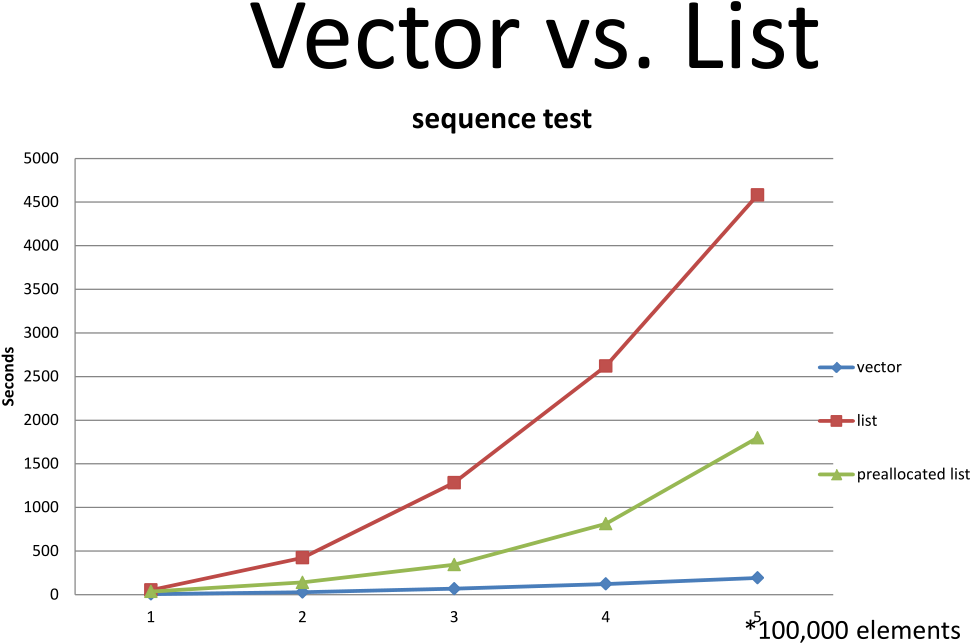
\includegraphics[scale=0.25]{VS.png}}
\end{center}
\end{frame}

\begin{frame}
\frametitle{Modèle académique}
\begin{center}
\begin{tikzpicture}[-,>=stealth',shorten >=1pt,auto,node distance=3cm,
  thick,main node/.style={circle,draw,font=\sffamily\Large\bfseries}]
            
    \draw[white] (0, 0) -- (1, 1) -- (9, 1) -- (10, 0) -- (0, 0);
    
    \draw[white] (4, 5) -- (5, 6) -- (6, 5) -- (4, 5);
    
    \draw[white] (5, 1) -- (5, 5);
\end{tikzpicture}
\end{center}

\begin{textblock}{5}(7, 13.1)
	 Mémoire
\end{textblock}
\begin{textblock}{5}(7.5, 5)
	 CPU
\end{textblock}
\end{frame}

\begin{frame}
\frametitle{Réalité}
\begin{center}
\begin{tikzpicture}[-,>=stealth',shorten >=1pt,auto,node distance=3cm,
  thick,main node/.style={circle,draw,font=\sffamily\Large\bfseries}]
            
    \draw[white] (0, 0) -- (1, 1) -- (9, 1) -- (10, 0) -- (0, 0);
    
    \draw[white] (1, 1.25) -- (2, 2.25) -- (8, 2.25) -- (9, 1.25) -- (1, 1.25);
    
    \draw[white] (2, 2.5) -- (3, 3.5) -- (7, 3.5) -- (8, 2.5) -- (2, 2.5);
    
    \draw[white] (3, 3.75) -- (4, 4.75) -- (6, 4.75) -- (7, 3.75) -- (3, 3.75);
    
    \draw[white] (4, 5) -- (5, 6) -- (6, 5) -- (4, 5);
    
    \draw[white] (5, 1) -- (5, 1.25);
    \draw[white] (5, 2.25) -- (5, 2.5);
    \draw[white] (5, 3.5) -- (5, 3.75);
    \draw[white] (5, 4.75) -- (5, 5);
\end{tikzpicture}
\end{center}

\begin{textblock}{5}(7, 13.1)
	 Mémoire
\end{textblock}
\begin{textblock}{5}(7, 11)
	 Cache L3
\end{textblock}
\begin{textblock}{5}(7, 9)
	 Cache L2
\end{textblock}
\begin{textblock}{5}(7, 7)
	 Cache L1
\end{textblock}
\begin{textblock}{5}(7.5, 5)
	 CPU
\end{textblock}
\end{frame}

\begin{frame}
\frametitle{Architecture multi-coeurs}
\begin{itemize}
\item Plus de coeurs veut souvent dire réduction de la taille de cache par coeurs
\item Mauvaise gestion de la cache peut faire perdre tous les gains potentiels du parallélisme
\end{itemize}
\end{frame}

\section{Fonctionnement de la cache}
\subsection{Concepts de base}
\begin{frame}
\frametitle{Accès à la mémoire}
\begin{itemize}
\item En général, les processeurs ne peuvent accéder directement à la mémoire
\item Les accès mémoire se font au travers d'une hiérarchie de caches
\item Les lectures se font par blocs (\textit{cache lines})
\end{itemize}
\end{frame}

\begin{frame}
\frametitle{Cache}
\framesubtitle{Illustration}
\begin{columns}
    \begin{column}{0.7\textwidth}
\begin{center}
\begin{tikzpicture}[-,>=stealth',shorten >=1pt,auto,node distance=3cm,
  thick,main node/.style={circle,draw,font=\sffamily\Large\bfseries}]

    \draw[white] (0, 0) rectangle (4, 0.75);
    \draw[white] (0, 0.75) rectangle (4, 1.5);
    \draw[white] (0, 1.5) rectangle (4, 2.25);
    \draw[white] (0, 2.25) rectangle (4, 3);
    \draw[white] (0, 3) rectangle (4, 3.75);
    \draw[white] (0, 3.75) rectangle (4, 4.5);
    
    \draw[white] (-0.1, -0.03) -- (-0.3, -0.03) -- (-0.3, 4.5) -- (-0.1, 4.5) node (1) at (-0.7, 2.4) {$M$};
    
    \draw[white] (0, -0.1) -- (0, -0.3) -- (4, -0.3) -- (4, -0.1) node (1) at (2, -0.6) {$B$};
   
\end{tikzpicture}
\end{center}
    \end{column}
    \begin{column}{0.4\textwidth}
\begin{itemize}
\item Comporte $B$ blocs (\textit{cache lines})
\item Taille $M$
\item Chaque bloc à une taille $B/M$
\end{itemize}
    \end{column}
\end{columns}
\end{frame}

\begin{frame}[fragile]
\frametitle{Lecture}
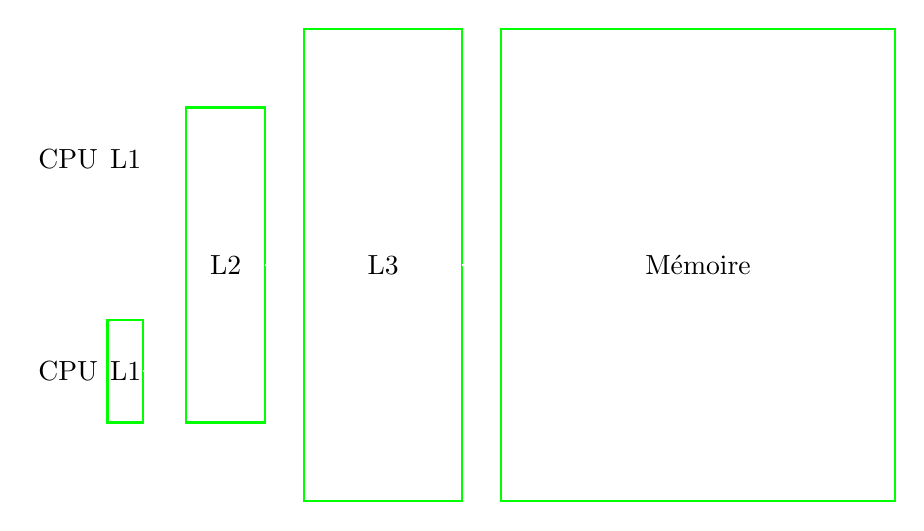
\begin{tikzpicture}[-,>=stealth',shorten >=1pt,auto,node distance=3cm,
  thick,main node/.style={circle,draw,font=\sffamily\Large\bfseries}]

	\draw[white] (0, 0) rectangle (1.45, 1.3);
	\draw[white] (1, 0) rectangle (1.45, 1.3);
	\onslide<2>{\draw[red] (1, 0) rectangle (1.45, 1.3);}
	\onslide<8->{\draw[green] (1, 0) rectangle (1.45, 1.3);}
	\draw[white] (0, 2.7) rectangle (1.45, 4);
	\draw[white] (1, 2.7) rectangle (1.45, 4);
	\draw[white] (2, 0) rectangle (3, 4);
	\onslide<3>{\draw[red] (2, 0) rectangle (3, 4);}
	\onslide<7->{\draw[green] (2, 0) rectangle (3, 4);}
	\draw[white] (3.5, -1) rectangle (5.5, 5);
	\onslide<4>{\draw[red] (3.5, -1) rectangle (5.5, 5);}
	\onslide<6->{\draw[green] (3.5, -1) rectangle (5.5, 5);}
    \draw[white] (6, -1) rectangle (11, 5);
    \onslide<5->{\draw[green] (6, -1) rectangle (11, 5);}
    
    \node (1) at (0.5, 0.65) {CPU};
    \node (2) at (0.5, 3.35) {CPU};
    \node (3) at (1.23, 0.65) {L1};
    \node (4) at (1.23, 3.35) {L1};
    \node (5) at (2.5, 2) {L2};
    \node (6) at (4.5, 2) {L3};
    \node (7) at (8.5, 2) {Mémoire};
    
    \draw[white] (1.45, 0.65) -- (2, 0.65);
    \draw[white] (1.45, 3.35) -- (2, 3.35);
    \draw[white] (3, 2) -- (3.5, 2);
    \draw[white] (5.5, 2) -- (6, 2);

\end{tikzpicture}
\begin{textblock}{6}(2.5, 4)
	\begin{lstlisting}
		LOAD X
	\end{lstlisting}
\end{textblock}
\end{frame}

\begin{frame}
\frametitle{Écriture}
Deux approches:
\begin{itemize}
\item \textit{Write-through}
\item \textit{Write-back}
\end{itemize}
\end{frame}

\begin{frame}
\frametitle{\textit{Write-through}}
\begin{itemize}
\item Le contenu de la cache et de la mémoire sont mis à jour simultanément
\item Le contenu de chaque cache est identique au contenu de la mémoire en tout temps
\item Minimise la perte de données
\end{itemize}
\end{frame}

\begin{frame}
\frametitle{\textit{Write-back}}
\begin{itemize}
\item La mise à jour de la mémoire est différée à des moments précis
\begin{itemize}
\item Exemple: Lecture de l'emplacement mémoire, \textit{cache line} sur le point de se faire évincer
\end{itemize}
\item Offre des gains de performance en vitesse
\end{itemize}
\end{frame}

\subsection{Cohérence}
\begin{frame}
\frametitle{Problème}
\begin{center}
\LARGE{Que se passe-t-il dans un contexte parallèle?}
\end{center}
\end{frame}

\begin{frame}
\frametitle{Protocole de cohérence}
Assurer que le contenu de multiples caches demeurent cohérent
\begin{itemize}
\item Toutes les écritures sont éventuellement vues par une lecture
\item Ordonnancement des écritures
\end{itemize}

Deux grandes familles de protocole
\begin{itemize}
\item Cohérence par répertoire
\item Cohérence par espionnage
\end{itemize}
\end{frame}

\begin{frame}
\frametitle{Cohérence par répertoire}
\begin{itemize}
\item Répertoire central conservant des informations sur ce qui est partagé
\item Messages inter-processeurs pour faire la requête de données
\item \textit{Scale} mieux
\end{itemize}
\end{frame}

\begin{frame}
\frametitle{Cohérence par espionnage}
\framesubtitle{Concept}
\begin{itemize}
\item Tout les processeurs espionnent le bus
\item Une seule cache effectue une lecture ou une écriture en mémoire dans un cycle donné
\item Que faire avec écriture de type \textit{write-back}?
\end{itemize}
\end{frame}

\begin{frame}
\frametitle{Protocole MESI}
\framesubtitle{Définitions}
4 états possibles: 
\begin{itemize}
\item[M] $\rightarrow$ Modifié: Copie modifiée d'une valeur en mémoire
\item[E] $\rightarrow$ Exclusif: Copie propre d'une donnée en mémoire présente uniquement dans la cache courante
\item[S] $\rightarrow$ Partagé: Copie propre d'une donnée en mémoire que plusieurs caches peuvent posséder
\item[I] $\rightarrow$ Invalide: Ne peut être utilisée
\end{itemize}
\end{frame}

\begin{frame}
\frametitle{Protocole MESI}
\framesubtitle{Illustration}
\begin{center}
\resizebox{5.9cm}{!}{
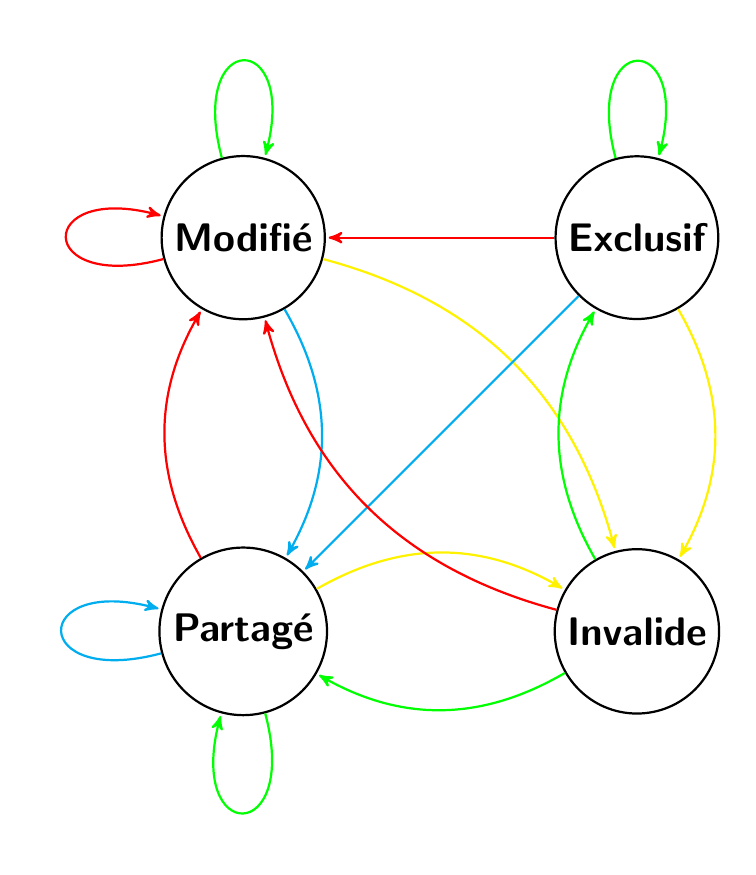
\begin{tikzpicture}[-,>=stealth',shorten >=1pt,auto,node distance=5cm,
  thick,main node/.style={circle,draw,font=\sffamily\Large\bfseries}]

	\node[main node] (1) {Modifié};
    \node[main node] (2) [right of=1] {Exclusif};
    \node[main node] (3) [below of=1] {Partagé};
    \node[main node] (4) [right of=3] {Invalide};
    
    \path (1) edge [cyan, ->, bend left] (3);
    \path (1) edge [yellow, ->, bend left] (4);
    \path (1) edge [green, ->, loop above] (1);
    \path (1) edge [red, ->, loop left] (1);
    \path (2) edge [green, ->, loop above] (2);
    \path (2) edge [red, ->] (1);
    \path (2) edge [cyan, ->] (3);
    \path (2) edge [yellow, ->, bend left] (4);
    \path (3) edge [red, ->, bend left] (1);
    \path (3) edge [yellow, ->, bend left] (4);
    \path (3) edge [cyan, ->, loop left] (3);
    \path (3) edge [green, ->, loop below] (3);
    \path (4) edge [red, ->, bend left] (1);
    \path (4) edge [green, ->, bend left] (2);
    \path (4) edge [green, ->, bend left] (3);

\end{tikzpicture}
}
\end{center}
\begin{textblock}{5}(1, 7.8)
\textcolor{red}{Écriture locale} \\
\textcolor{green}{Lecture locale} \\
\textcolor{cyan}{Lecture distante} \\
\textcolor{yellow}{Écriture distante}
\end{textblock}
\end{frame}


\begin{frame}
\frametitle{Protocole MESI}
\framesubtitle{Grandes lignes}
L'important à retenir est:
\begin{enumerate}
\item Pour écrire, un coeur doit obtenir un accès exclusif pour écrire dans une \textit{cache line}
\item Pour lire, un coeur doit faire passer l'état d'une \textit{cache line} à l'état \textit{Partagé}
\end{enumerate}

\only<2>{
\textbf{Pour être performant, il faut lire et écrire le plus localement possible }
}
\end{frame}

\section{Modèle insensible à la cache}
\subsection{Concept}
\begin{frame}
\frametitle{Concept}
\begin{columns}
    \begin{column}{0.5\textwidth}
\begin{itemize}
\item Conscience de l'existence d'une cache
\item Inconscience des détails spécifiques
\end{itemize}
    \end{column}
    \begin{column}{0.5\textwidth}
\begin{center}
\begin{tikzpicture}[-,>=stealth',shorten >=1pt,auto,node distance=3cm,
  thick,main node/.style={circle,draw,font=\sffamily\Large\bfseries}]

    \draw[white] (0, 0) rectangle (4, 0.75);
    \draw[white] (0, 0.75) rectangle (4, 1.5);
    \draw[white] (0, 1.5) rectangle (4, 2.25);
    \draw[white] (0, 2.25) rectangle (4, 3);
    \draw[white] (0, 3) rectangle (4, 3.75);
    \draw[white] (0, 3.75) rectangle (4, 4.5);
    
    \draw[white] (-0.1, -0.03) -- (-0.3, -0.03) -- (-0.3, 4.5) -- (-0.1, 4.5) node (1) at (-0.7, 2.4) {$M$};
    
    \draw[white] (0, -0.1) -- (0, -0.3) -- (4, -0.3) -- (4, -0.1) node (1) at (2, -0.6) {$B$};
   
\end{tikzpicture}
\end{center}
    \end{column}
\end{columns}
\end{frame}

\subsection{Algorithme}
\begin{frame}
\frametitle{Algorithmes insensibles à la cache}
\begin{itemize}
\item Réduire la taille des données traitées pour qu'elles rentrent en cache
\item Doit profiter de la hiérarchie mémoire d'une machine peu importe ces caractéristiques
\item Algorithmes souvent récursifs
\end{itemize}
\end{frame}

\begin{frame}[fragile]
\frametitle{Élimination de la récursion}
Les compilateurs modernes comprennent la récursivité et peuvent l'optimiser dans certains cas. Par exemple:
\\
\begin{columns}
    \begin{column}{0.6\textwidth}
    \footnotesize{
    \begin{lstlisting}
int factorial(int x) {
  if(x > 1)
    return x * factorial(x-1);
  else return 1;
}
\end{lstlisting}}
    \end{column}
    \begin{column}{0.4\textwidth}
    \footnotesize{
    \begin{lstlisting}
int factorial(int x) {
  in result = 1;
  while(x > 1)
    result *= x--;
  return result;
}
\end{lstlisting}}
    \end{column}
\end{columns}
\begin{textblock}{5}(8.7, 9.5)
	 \Huge{$\Rightarrow$}
\end{textblock}
\end{frame}

\begin{frame}[fragile]
\frametitle{Multiplication de matrices}
\framesubtitle{Approche traditionnelle}
\begin{lstlisting}
for (int i = 0; i < N; ++i)
  for (int j = 0; j < N; ++i)
    for (int k = 0; k < N; ++k)
      C[i][j] += A[i][k] * B[k][j];
\end{lstlisting}

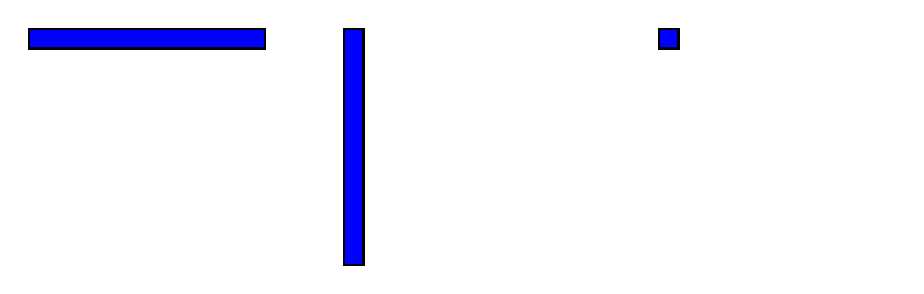
\begin{tikzpicture}[-,>=stealth',shorten >=1pt,auto,node distance=3cm,
  thick,main node/.style={circle,draw,font=\sffamily\Large\bfseries}]

    \draw[white] (0, 0) rectangle (3, 3);
    \draw[white] (4, 0) rectangle (7, 3);
    \draw[white] (8, 0) rectangle (11, 3);
    
    \draw[fill=blue] (0, 2.75) rectangle (3, 3);
    \draw[fill=blue] (4, 0) rectangle (4.25, 3);
    \draw[fill=blue] (8, 2.75) rectangle (8.25, 3);
 
\end{tikzpicture}

\begin{textblock}{5}(5.25, 11)
	 \Huge{$\times$}
\end{textblock}

\begin{textblock}{5}(10.25, 11.2)
	 \Huge{$=$}
\end{textblock}
\end{frame}

\begin{frame}[fragile]
\frametitle{Multiplication de matrices}
\framesubtitle{Approche optimisée}
\begin{lstlisting}
for (int i = 0; i < N; ++i)
  for (int j = 0; j < N; ++i)
      B[i][j] = B[j][i];
for (int i = 0; i < N; ++i)
  for (int j = 0; j < N; ++i)
    for (int k = 0; k < N; ++k)
      C[i][j] += A[i][k] * B[j][k];
\end{lstlisting}

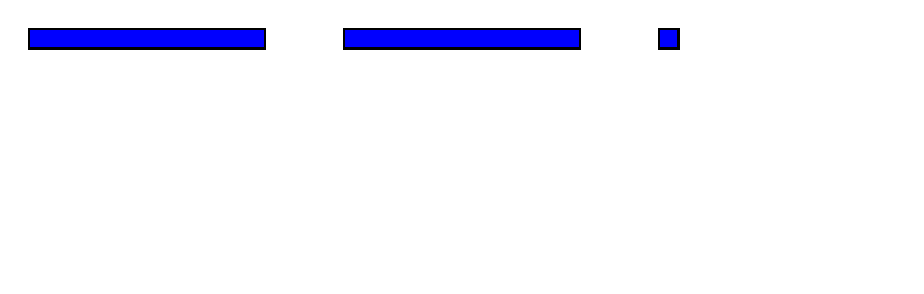
\begin{tikzpicture}[-,>=stealth',shorten >=1pt,auto,node distance=3cm,
  thick,main node/.style={circle,draw,font=\sffamily\Large\bfseries}]

    \draw[white] (0, 0) rectangle (3, 3);
    \draw[white] (4, 0) rectangle (7, 3);
    \draw[white] (8, 0) rectangle (11, 3);
    
    \draw[fill=blue] (0, 2.75) rectangle (3, 3);
    \draw[fill=blue] (4, 2.75) rectangle (7, 3);
    \draw[fill=blue] (8, 2.75) rectangle (8.25, 3);
 
\end{tikzpicture}

\begin{textblock}{5}(5.25, 12)
	 \Huge{$\times$}
\end{textblock}

\begin{textblock}{5}(10.25, 12.2)
	 \Huge{$=$}
\end{textblock}
\end{frame}

\begin{frame}[fragile]
\frametitle{Multiplication de matrices}
\framesubtitle{Approche insensible à la cache}
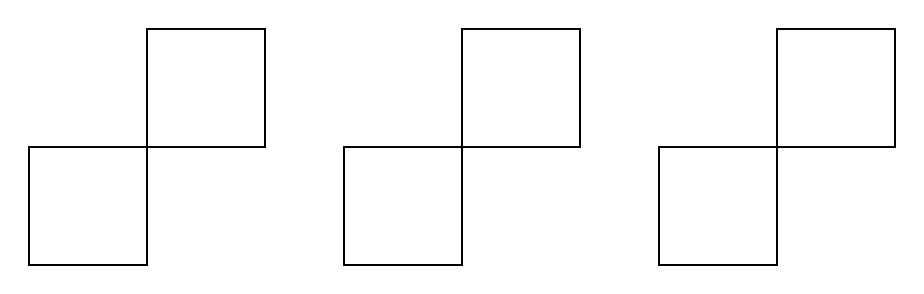
\begin{tikzpicture}[-,>=stealth',shorten >=1pt,auto,node distance=3cm,
  thick,main node/.style={circle,draw,font=\sffamily\Large\bfseries}]

    \draw[white] (0, 0) rectangle (3, 3);
    \draw[white] (4, 0) rectangle (7, 3);
    \draw[white] (8, 0) rectangle (11, 3);
    
    \draw (0, 0) rectangle (1.5, 1.5);
    \draw (1.5, 1.5) rectangle (3, 3);    
    
    \draw (4, 0) rectangle (5.5, 1.5);
    \draw (5.5, 1.5) rectangle (7, 3);
    
    \draw (8, 0) rectangle (9.5, 1.5);
    \draw (9.5, 1.5) rectangle (11, 3);
     
\end{tikzpicture}

\begin{textblock}{5}(1.65, 7.1)
	 \Huge{A1}
\end{textblock}

\begin{textblock}{5}(1.65, 9.6)
	 \Huge{A2}
\end{textblock}

\begin{textblock}{5}(3.5, 7.1)
	 \Huge{A3}
\end{textblock}

\begin{textblock}{5}(3.5, 9.6)
	 \Huge{A4}
\end{textblock}

\begin{textblock}{5}(6.65, 7.1)
	 \Huge{B1}
\end{textblock}

\begin{textblock}{5}(6.65, 9.6)
	 \Huge{B2}
\end{textblock}

\begin{textblock}{5}(8.5, 7.1)
	 \Huge{B3}
\end{textblock}

\begin{textblock}{5}(8.5, 9.6)
	 \Huge{B4}
\end{textblock}

\begin{textblock}{1}(11.55, 5.6)
\begin{center}
A1xB1 + A2xB3
\end{center}	 
\end{textblock}

\begin{textblock}{1}(11.55, 8.1)
\begin{center}
	 A1xB2 + A2xB4
	 \end{center}	
\end{textblock}

\begin{textblock}{1}(13.45, 5.6)
\begin{center}
	 A3xB1 + A4xB3
	 \end{center}	
\end{textblock}

\begin{textblock}{1}(13.45, 8.1)
\begin{center}
	 A3xB2 + A4xB4
	 \end{center}	
\end{textblock}

\begin{textblock}{5}(5.25, 8.5)
	 \Huge{$\times$}
\end{textblock}

\begin{textblock}{5}(10.25, 8.7)
	 \Huge{$=$}
\end{textblock}

\end{frame}


\begin{frame}
\frametitle{Comparaison}
\framesubtitle{Mise en contexte}
\begin{itemize}
\item Test séquentiel
\item Matrices de taille $N \times N$
\item Processeur: Intel Core i5-4670
\item Compilateur: g++ 4.8.3
\item Option d'optimisation: -O2
\end{itemize}
\end{frame}

\begin{frame}
\frametitle{Comparaison}
\framesubtitle{Résultats personnels}
\begin{center}
\colorbox{white}{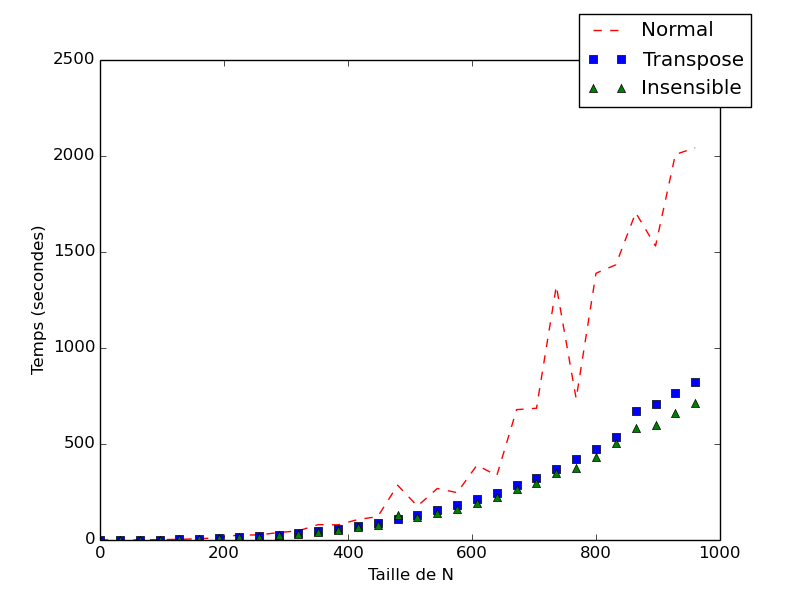
\includegraphics[scale=0.4]{matmult_all.png}}
\end{center}
\end{frame}

\begin{frame}
\frametitle{Comparaison}
\framesubtitle{Résultats personnels}
\begin{center}
\colorbox{white}{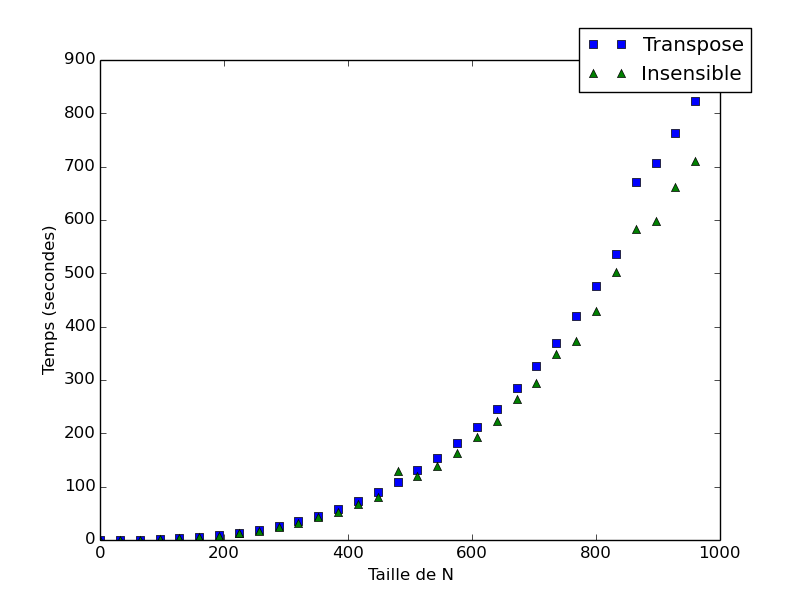
\includegraphics[scale=0.4]{matmult.png}}
\end{center}
\end{frame}

\begin{frame}
\frametitle{Comparaison}
\framesubtitle{CARMA}
\begin{itemize}
\item Tests en mémoire partagée sur 4 Intel Xeon X7560 totalisant 32 coeurs
\item Parallélisé avec Cilk Plus
\item Matrices de taille: $64 \times k \times 64$
\item Comparaison avec Intel MKL
\end{itemize}
\end{frame}

\begin{frame}
\frametitle{Comparaison}
\framesubtitle{Résultats CARMA}
\begin{center}
\colorbox{white}{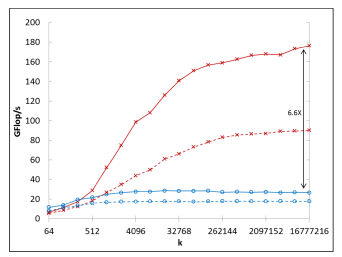
\includegraphics[scale=0.9]{CARMA.png}}
\end{center}
\end{frame}

\begin{frame}
\frametitle{Plus sur le sujet}
\framesubtitle{Algorithmes}
\begin{itemize}
\item \textit{Funnelsort}
\item Parcours de séquences (map, filter, etc...)
\item Calcul matriciel
\end{itemize}
\end{frame}

\begin{frame}
\frametitle{Plus sur le sujet}
\framesubtitle{Structures de données}
\begin{itemize}
\item Liste déroulée
\item Arbre de van Emde Boas
\item Matrices récursives
\end{itemize}
\end{frame}

\section{Conclusion}
\begin{frame}
\frametitle{Conclusion}
\begin{itemize}
\item La cohérence des caches d'un système est assuré par le matériel.
\item<2-> Une façon d'exploiter la localité est d'utiliser des algorithmes et des structures de données insensibles à la cache.
\item<3-> Les algorithmes insensibles à la cache offrent des opportunités de parallélisation.
\end{itemize}
\end{frame}

\end{document}